\documentclass[../../main.tex]{subfiles}
\graphicspath{{images/Maschinentechnik/}{../../images/Maschinentechnik/}}

\begin{document}
    \subsection{Konzeptbeschreibung}
    Die Lokomotive in Abbildung ist in die drei Unterbaugruppen Antriebswagen (Position 1), Führungswagen (Position 2) und Ladungsträger (Position 3) unterteilt. Der Antriebswagen enthält alle notwendigen Komponenten, um die Lokomotive zu beschleunigen und wieder abzubremsen. Zusätzlich sind die Kameras für die Spur- und Signalerkennung an ihm angebracht. Der Führungswagen hingegen dient lediglich als Abstützung für den Ladungsträger. Er bietet aber zusätzlichen Bauraum für elektronische Komponenten. In den nachfolgenden Abschnitten wird auf die verschiedenen Unterbaugruppen eingegengen und vorgestellt.

    \begin{figure}[H] %Lokomotive mit Positionsnummern
        \centering
        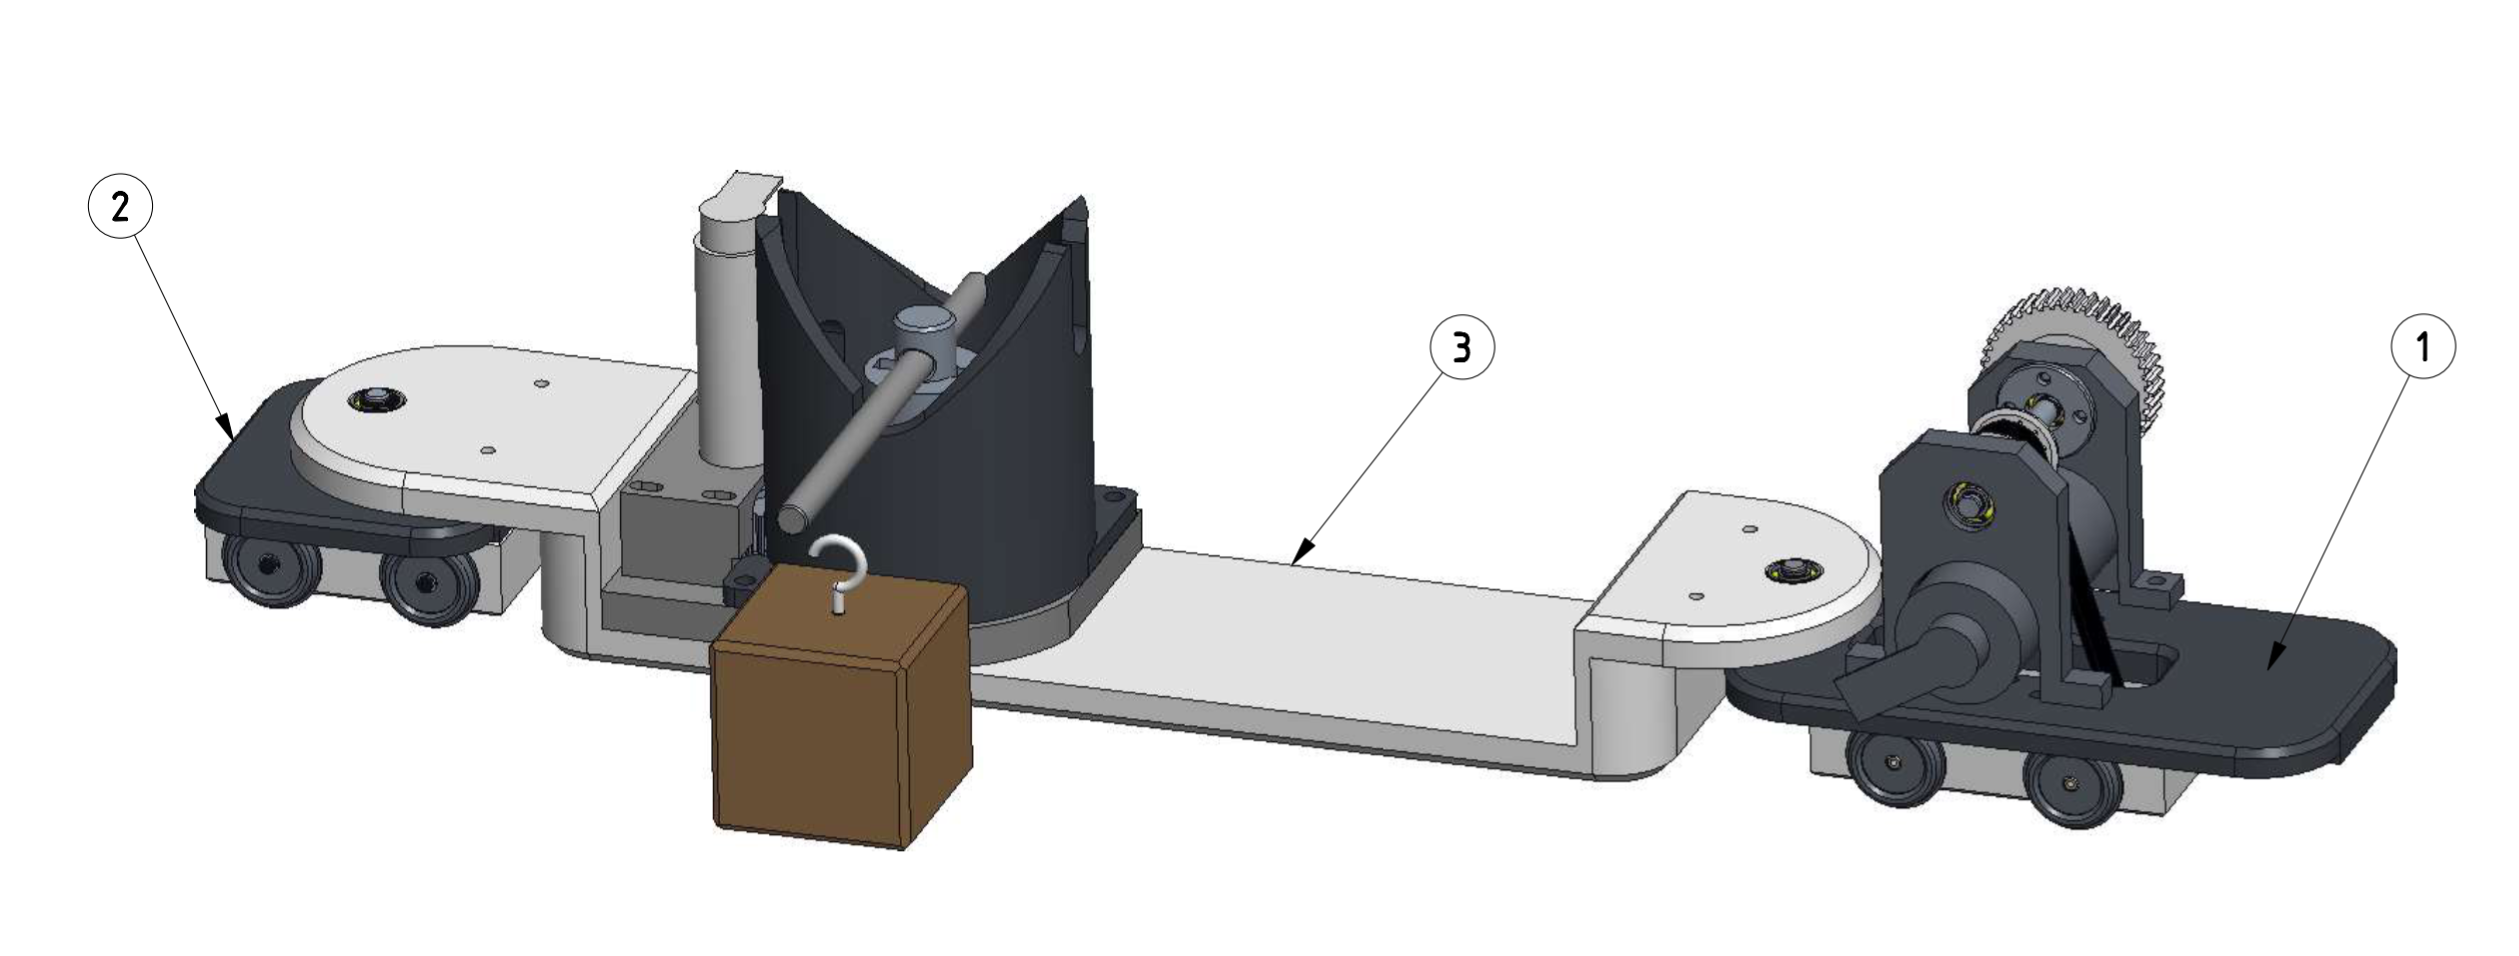
\includegraphics[width=0.9\textwidth]{Lokomotive.png}
        \caption{Baugruppe Lokomotive}
        \label{fig:bg_lokomotive}
    \end{figure}

    \begin{table}[H] \centering
        \begin{tabular}{|l|l|}
        \hline
        \textbf{Position} & \textbf{Bezeichnung}\\
        \hline
        Position 1          & Antriebswagen\\
         \hline
        Position 2          & Führungswagen\\
        \hline
        Position 3          & Ladungsträger\\
        \hline
        \end{tabular}

    \subsubsection{Antriebswagen}
    Der Grundaufbau der beiden Wägen ist derselbe, mit dem Unterschied, dass der Antriebswagen durch einen Motor angetrieben wird. Der Grundwagen beziehungsweise der Führungswagen in Abbildung besteht aus einem Rahmen und einer Platte, welche miteinander verstiftet (Position 2) und verschraubt (Position 3) sind. Im Rahmen werden die beiden Achsen jeweils mit einem Los- und einem Festlager lagert. Die Achsen sind an beiden Enden mit einem Gewinde versehen, damit die Räder bei Bedarf schnell und einfach gewechselt werden können, ohne dass der ganze Wagen auseinander genommen werden muss. Die Anfräsfläche auf der Welle (Position 5) dient für das bessere Befestigen der Räder durch einen Gabelschlüssel.

     \begin{figure}[H] %Führungswagen
        \centering
        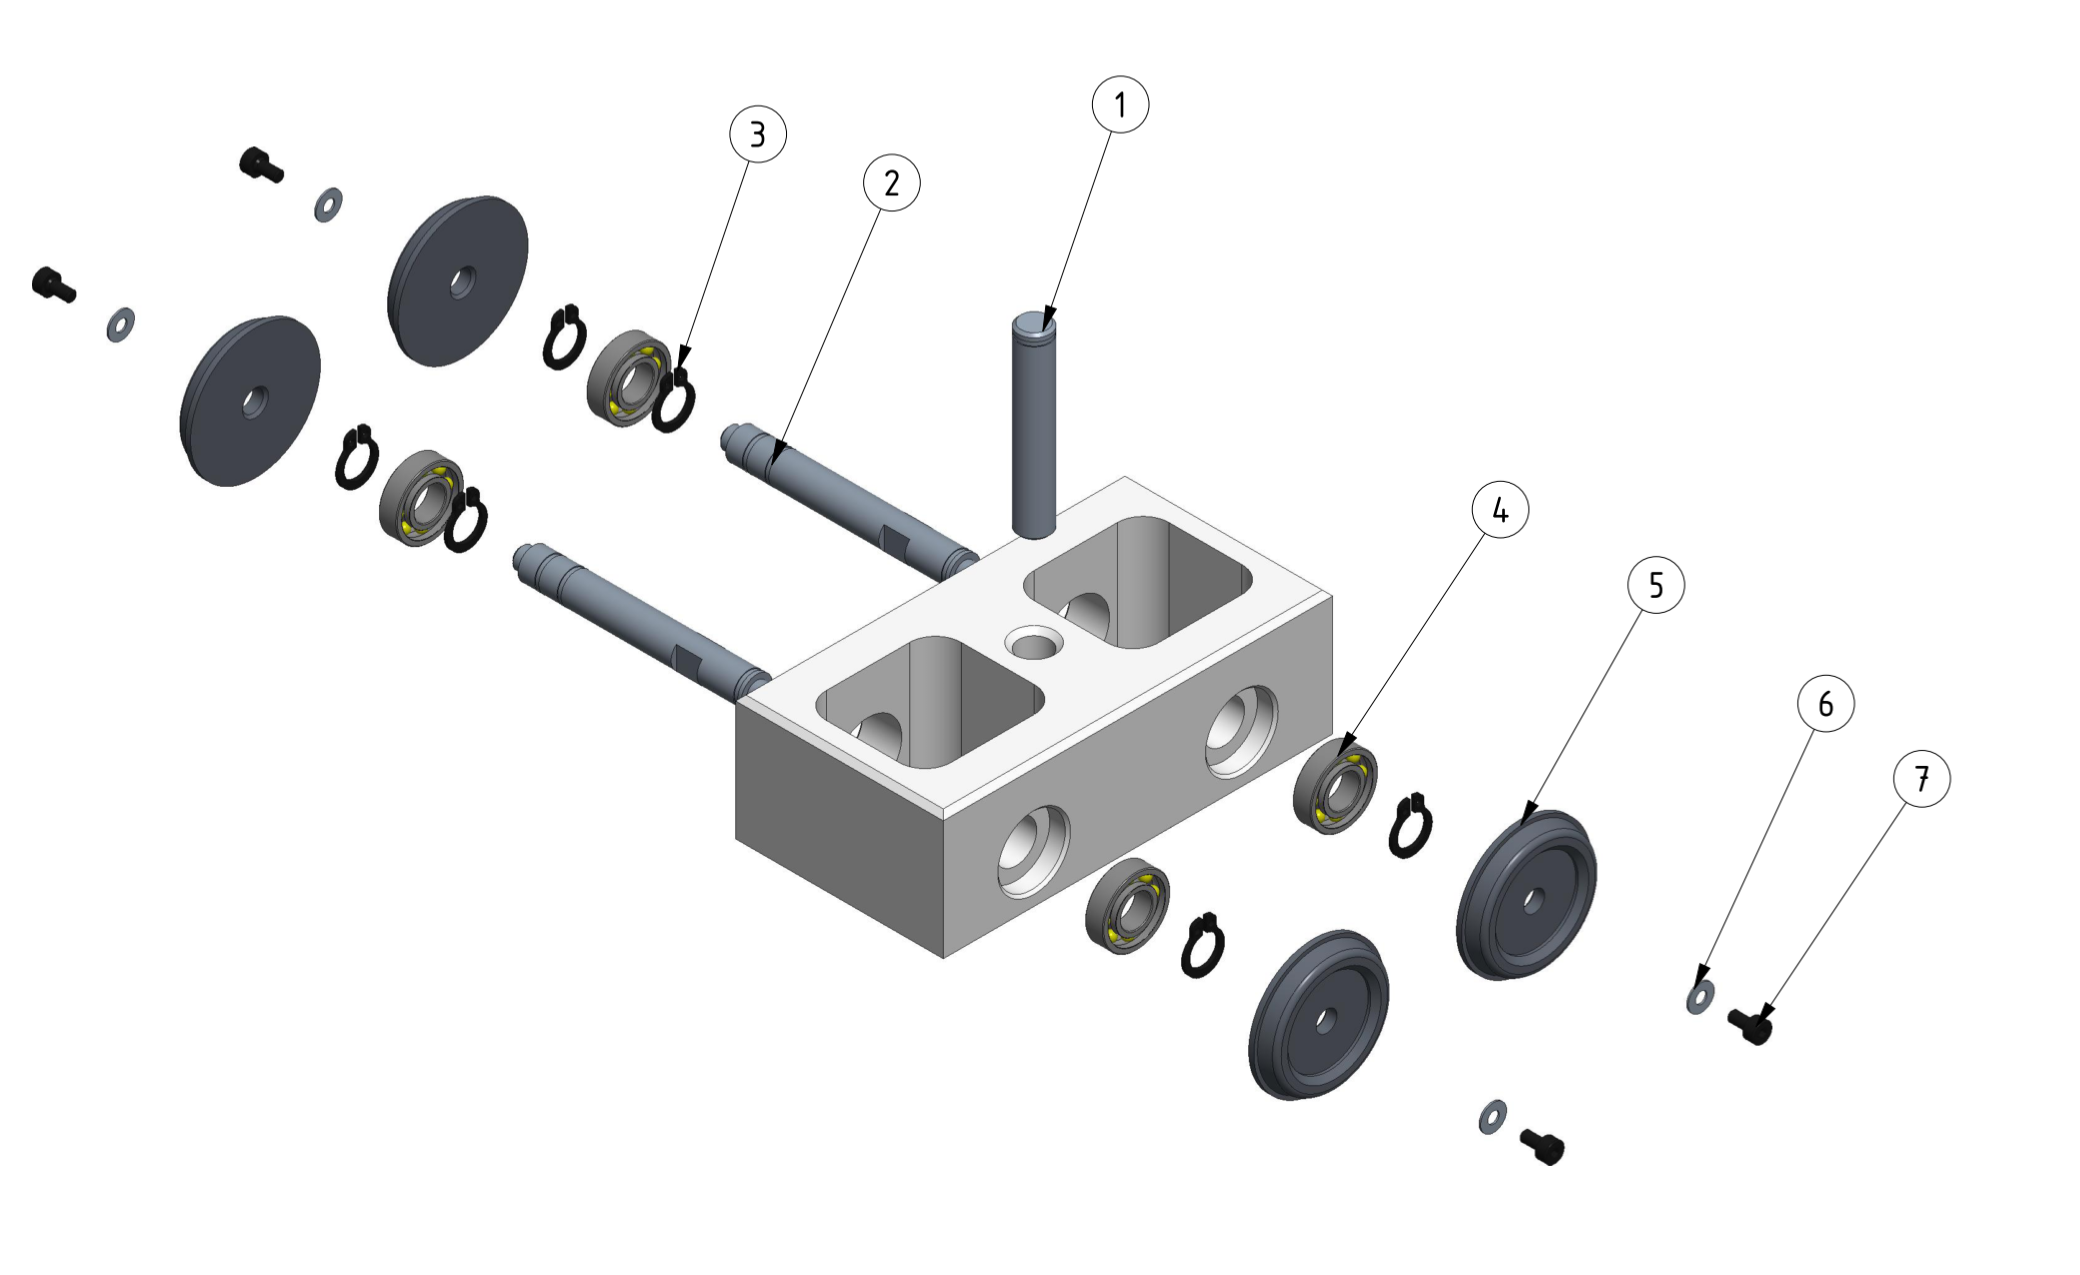
\includegraphics[width=0.9\textwidth]{Fuehrungswagen.png}
        \caption{Explosionsdarstellung Führungswagen}
        \label{fig:expl_fuehrungswagen}
    \end{figure}   

    \begin{table}[H] \centering
        \begin{tabular}{|l|l|}
        \hline
        \textbf{Position} & \textbf{Bezeichnung}\\
        \hline
        Position 1          & Drehachse Wagen-Ladungsträger\\
         \hline
        Position 2          & Stife für das Verstiften von Rahmen und Platte\\
        \hline
        Position 3          & Zylinderschrauben für das Befestigen der Platte am Rahmen\\
        \hline
        Position 4          & Platte\\
        \hline
        Position 5          & Achsen mit Gewinden an beiden Enden und Anfräsfläche für Gabelschlüssel\\
        \hline
        Position 6          & Sicherungsring für Rillenkugellager\\
        \hline
        Position 7          & Rillenkugellager (Loslager)\\
        \hline
        Position 8          & Eingepresstes Rillenkugellager (Festlager)\\
        \hline
        Position 9          & Rad\\
        \hline
        Position 10         & Unterlagscheibe\\
        \hline
        Position 11         & Zylinderschraube\\
        \hline
        \end{tabular}

    Der Antriebswagen in Abbildung ist grundsätzlich gleich aufgebaut wie der Führungswagen, jedoch ist der Rahmen aufgrund des Riemenantriebs etwas anders Aufgebaut. Die Platte, welche auf dem Rahmen angebracht ist, wurde grösser dimensioniert, damit  . 

    \begin{figure}[H] %Antriebswagen
        \centering
        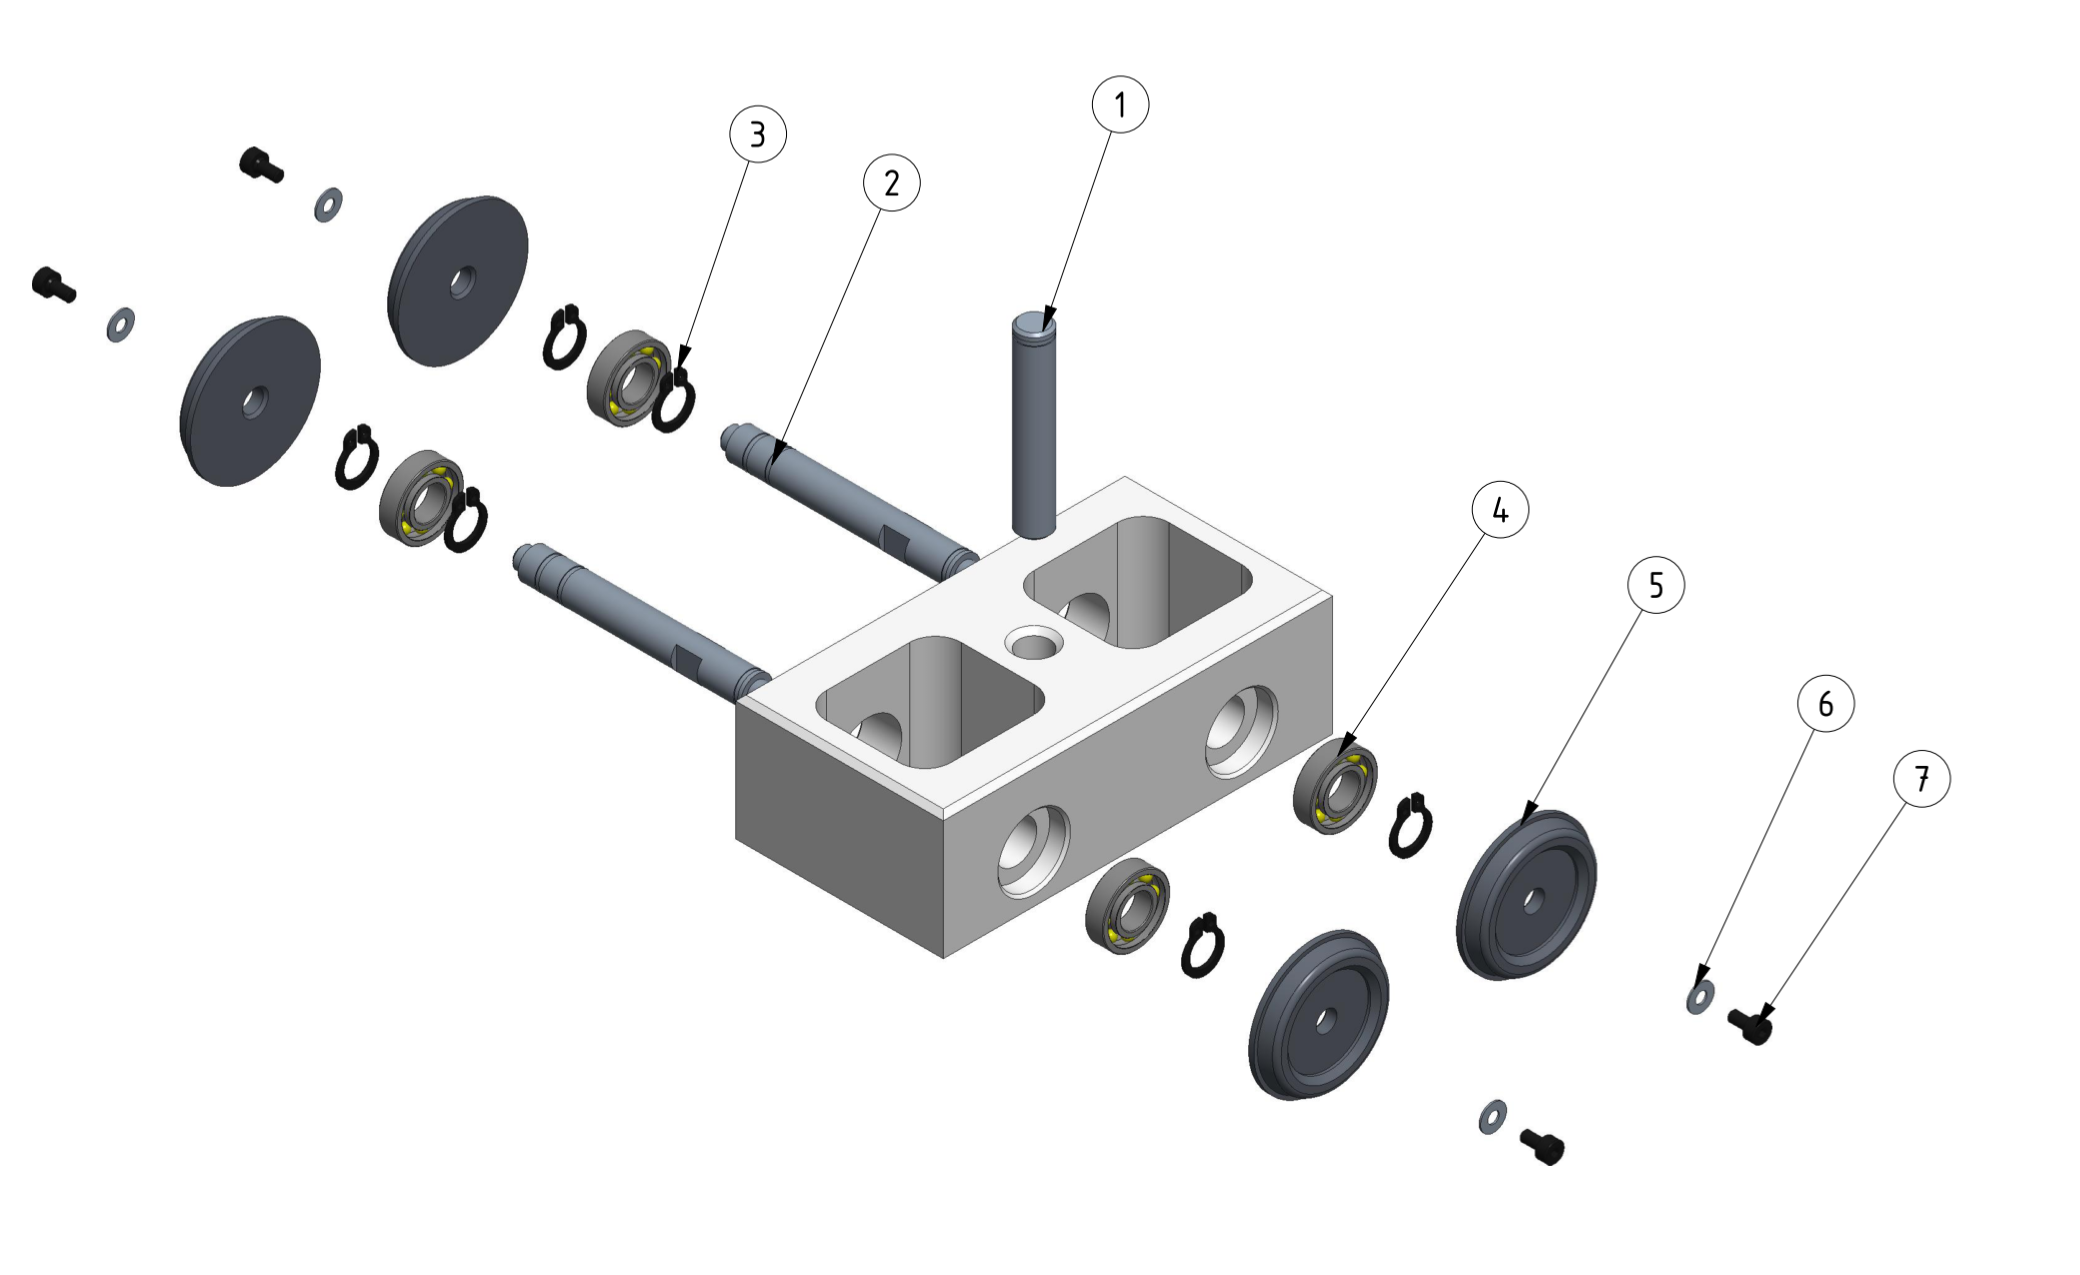
\includegraphics[width=0.9\textwidth]{Fuehrungswagen.png}
        \caption{Baugruppe Antriebswagen}
        \label{fig:Antriebswagen}
    \end{figure} 

    \begin{table}[H] \centering
        \begin{tabular}{|l|l|}
        \hline
        \textbf{Position} & \textbf{Bezeichnung}\\
        \hline
        Position 1          & Wagen\\
         \hline
        Position 2          & Antriebseinheit\\
        \hline
        \end{tabular}

    Antriebseinheit in Abbildung besteht aus einem Grundgestell, an welchem die Lagerung der Antriebswelle und der Motor angebracht sind. Das Drehmoment vom Motor wird über ein geradverzahntes Zahnrad mit einem Übersetzungsverhältnis von 1:2 auf eine Achse übertragen. Von dieser wird es über einen Riemen auf die beiden Radachsen und somit auf die Räder weitergeleitet. Durch die Berechnung der maximalen Geschwindigkeit wird entsprechend der Motor ausgelegt, was im nächsten Abschnitt genauer beschrieben wird.

    \begin{figure}[H] %Antriebseinheit
        \centering
        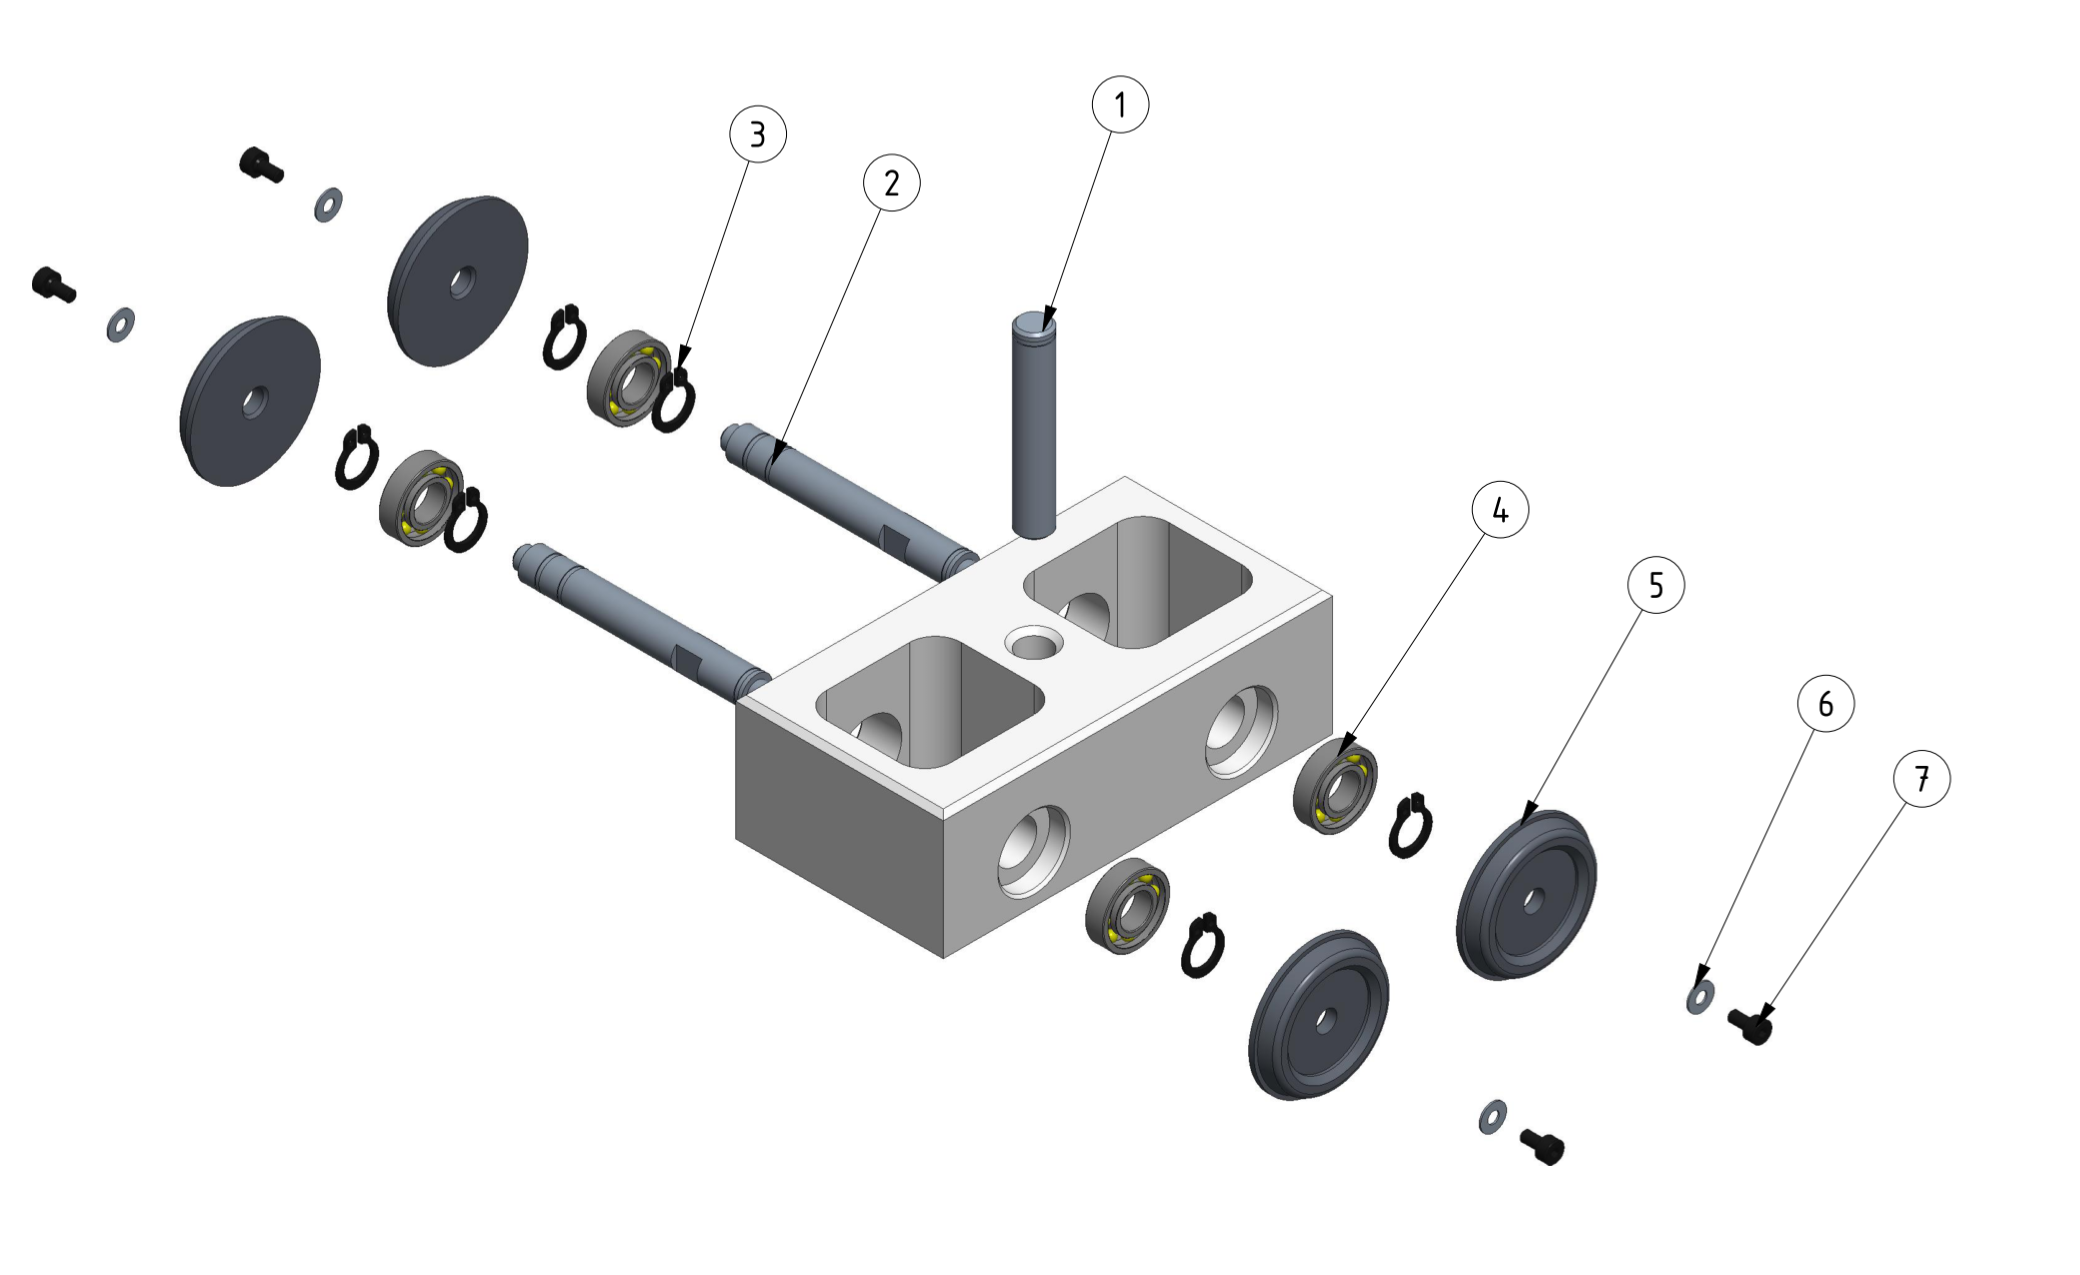
\includegraphics[width=0.9\textwidth]{Fuehrungswagen.png}
        \caption{Explosionsdarstellung Führungswagen}
        \label{fig:antriebseinheit}
    \end{figure} 

    \begin{table}[H] \centering
        \begin{tabular}{|l|l|}
        \hline
        \textbf{Position} & \textbf{Bezeichnung}\\
        \hline
        Position 1          & Drehachse Wagen-Ladungsträger\\
         \hline
        Position 2          & Stife für das Verstiften von Rahmen und Platte\\
        \hline
        Position 3          & Zylinderschrauben für das Befestigen der Platte am Rahmen\\
        \hline
        Position 4          & Platte\\
        \hline
        Position 5          & Achsen mit Gewinden an beiden Enden und Anfräsfläche für Gabelschlüssel\\
        \hline
        Position 6          & Sicherungsring für Rillenkugellager\\
        \hline
        Position 7          & Rillenkugellager (Loslager)\\
        \hline
        Position 8          & Eingepresstes Rillenkugellager (Festlager)\\
        \hline
        Position 9          & Rad\\
        \hline
        Position 10         & Unterlagscheibe\\
        \hline
        Position 11         & Zylinderschraube\\
        \hline
        \end{tabular}

    \textbf{Geschwindigkeitsberechnung}\\
    Die Fahrgeschwindigkeit der Lokomotive wird durch drei Faktoren bestimmt. Einerseits muss die maximale Geschwindigkeit der Anforderungsliste eingehalten werden und andererseits wird die Geschwindigkeit in der Kurvenfahrt durch den Schwerpunkt des Fahrzeuges und durch die maximale Haftreibkraft zwischen Schiene und Rad eingeschränkt.

    In der Anforderungsliste wurde eine minimale Geschwindigkeit von 0.5 Meter pro Sekunde festgelegt. Der begrenzende Faktor der Geschwindigkeit in der Kurve ist der Schwerpunkt der Lokomotive. Je tiefer dieser ist, umso schneller kann die Kurve abgefahren werden. Über die Zentripedalkraft und die Gewichtskraft der Lokomotive wird die Momentengleichung aufgestellt. 

    \begin{table}[H] \centering
        \begin{tabular}{|l|l|}
        \hline
        \textbf{Grösse} & \textbf{Wert}\\
        \hline
        Minimaler Radius                                 & 0.8 Meter\\
         \hline
        Masse                                            & 3 Kilogramm\\
        \hline
        Schwerpunkt in x-Achse (maximaler Wert)          & Meter\\
        \hline
        Schwerpunkt in y-Achse (maximaler Wert)          & Meter\\
        \hline
        \end{tabular}\\
   
        Die Zentripedalkraft und die Gewichtskraft sind wie folgt definiert:\\
    
    F\textsubscript{G}=\(m*g=3kg*9.81m/s^2=29.4N\)\\

    F\textsubscript{max z}=\(\frac{m*v^2}{r}\)=\(\frac{m*v^2}{r}\)\\
    
    Da das Drehmoment eine vektorielle Grösse ist, müssen die beiden entstehenden Momente am Drehpunkt "P" auf am Gleis zusammen Null ergeben beziehungsweise gleich gross sein, damit es "statisch" bestimmt ist. Die Berechnungen sind auf den kleinsten Kurvenradius ausgelegt, da dort die grössere Zentripedalkraft entsteht.\\

    F\textsubscript{max z}=\(\frac{F\textsubscript{G}*x+F\textsubscript{A}*a}{y}\)=\(\frac{F\textsubscript{G}*x+F\textsubscript{A}*a}{y}\)\\

    %Bild von Zug (Ansicht von vorne) mit Schwerpunkt und Positionsnummern
    
    Das Kippmoment wird durch den Aufbau der Lokomotive minimiert. Da der Schwerpunkt durch die beiden Wagen mehr in das Zentrum des Kreismittelpunktes rückt.
    
    Um möglichst viel Drehmoment auf das Rad zu übertragen, muss die Haftreibung maximiert werden, da die Beschleunigung davon abhängt. Die Reibungskoeffizienten wurden experimentell ermittelt. Dazu wurden verscheidene Materialen auf das Gleis gelegt und mit einer Federwage die Reibungskraft ermittelt. Der Versuch wurde mit den Materialien Kunstoff, Holz, Stahl und Gummi ausgeführt.

    \textbf{Motorauslegung}\\
    %Text von Schöni

    \subsubsection{Ladungsträger}
    Der Ladungsträger ist das Verbindungselement von Antriebswagen und Führungswagen. Er wird an beiden Enden drehbar mit Radialkugellager gelagert.

    Der Träger besteht aus drei Teilen (siehe Abbidlung). Der Hauptgrund ist die einfachere und kostengünstigere Herstellung.

    %Berechnung Kugellagerkräfte

    \begin{figure}[H] %Ladungsträger
        \centering
        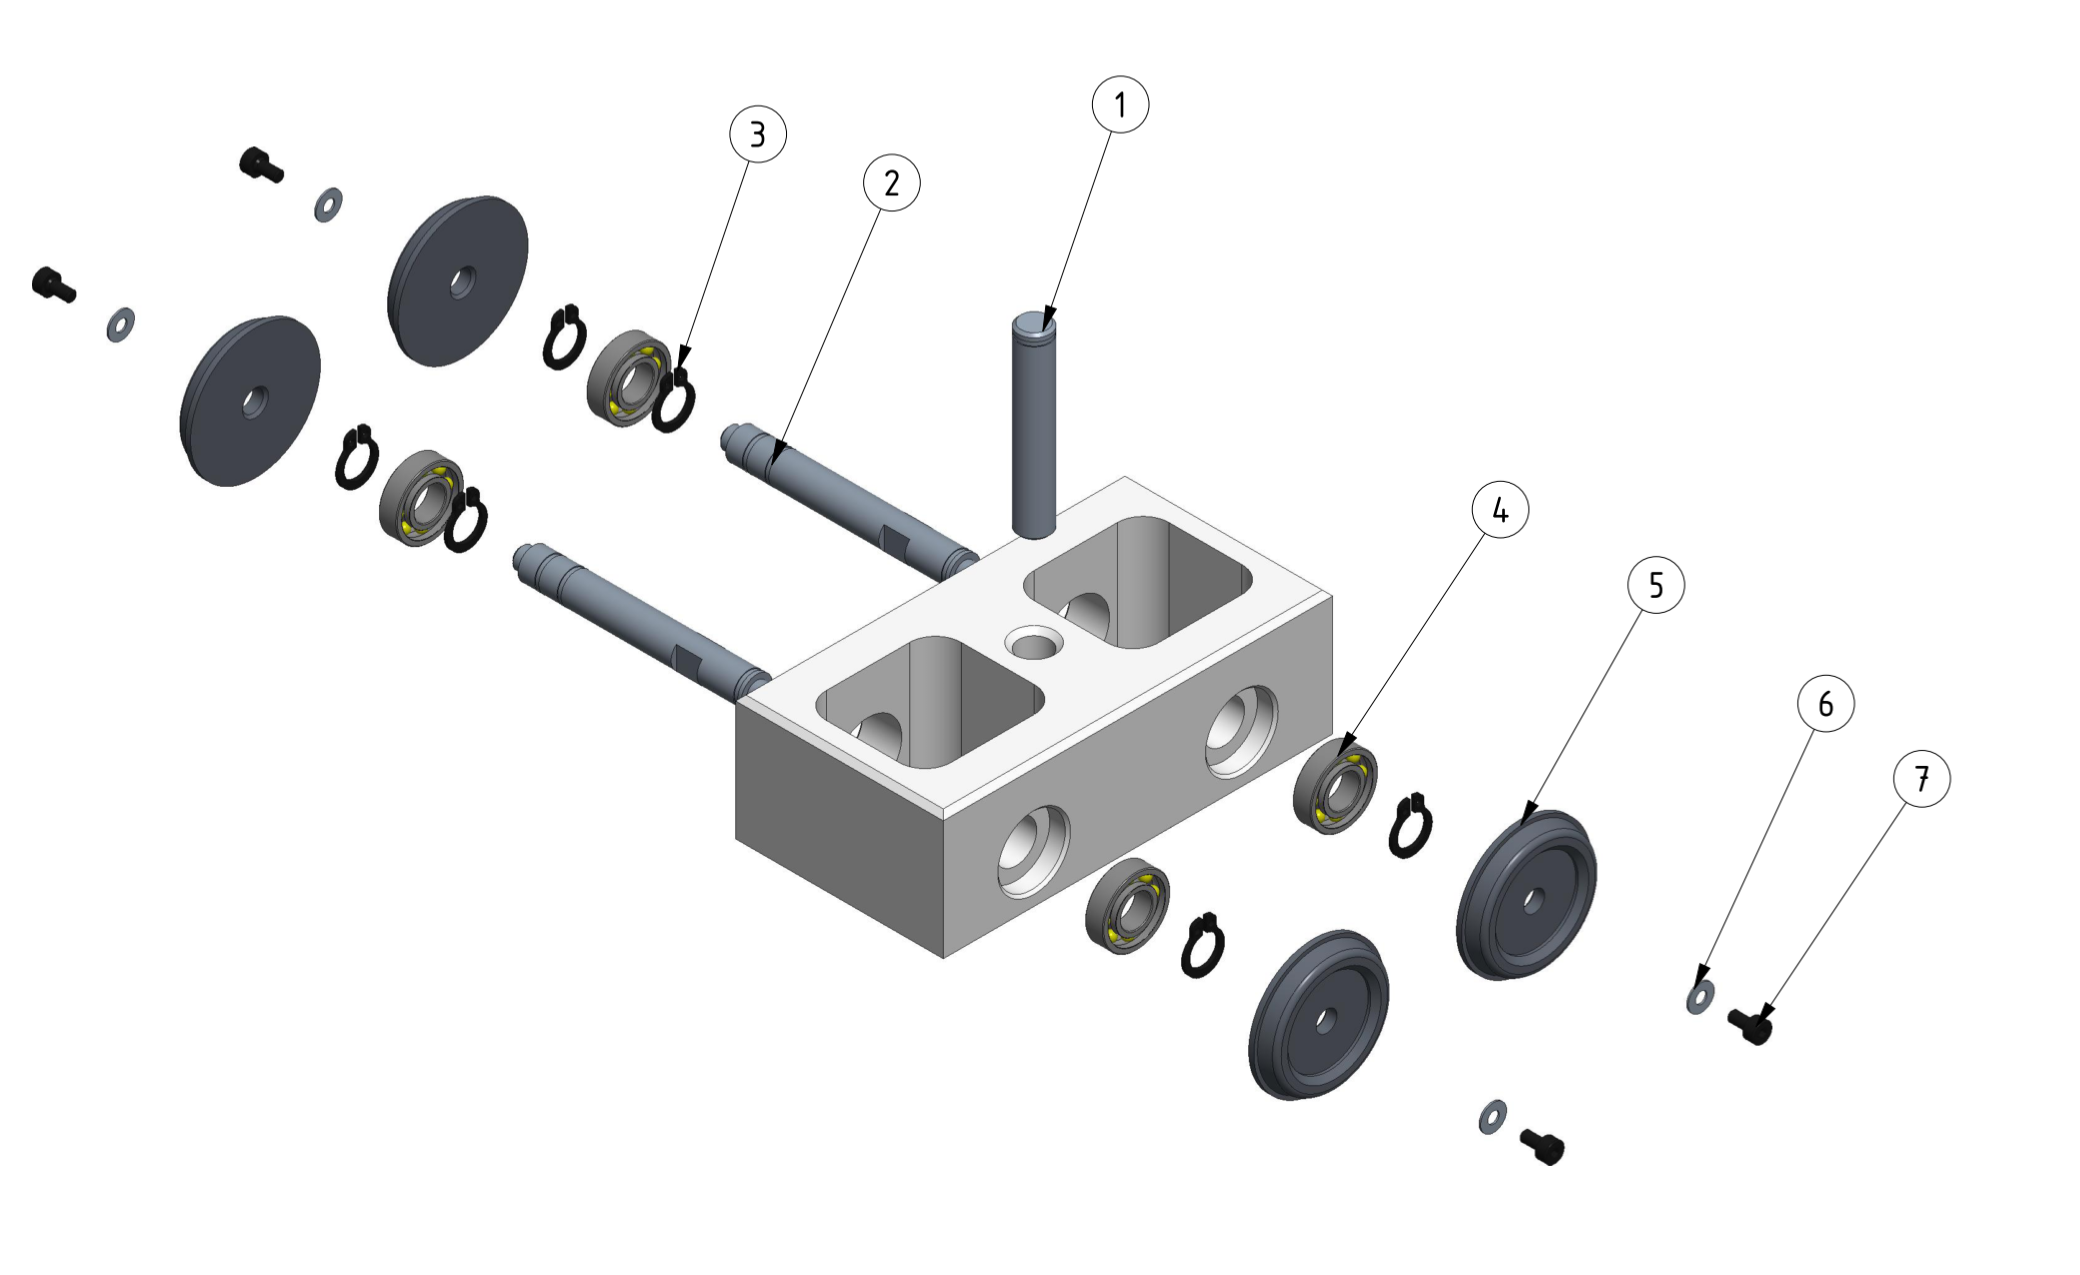
\includegraphics[width=0.9\textwidth]{Fuehrungswagen.png}
        \caption{Explosionsdarstellung Führungswagen}
        \label{fig:expl_fuehrungswagen}
    \end{figure}


    \begin{table}[H] \centering
        \begin{tabular}{|l|l|}
        \hline
        \textbf{Position} & \textbf{Bezeichnung}\\
        \hline
        Position 1          & Drehachse Wagen-Ladungsträger\\
         \hline
        Position 2          & Stife für das Verstiften von Rahmen und Platte\\
        \hline
        Position 3          & Zylinderschrauben für das Befestigen der Platte am Rahmen\\
        \hline
        Position 4          & Platte\\
        \hline
        Position 5          & Achsen mit Gewinden an beiden Enden und Anfräsfläche für Gabelschlüssel\\
        \hline
        \end{tabular}

    \textbf{Würfeltransport}\\
    %Text von Schöni
    
    \end{document}
